\chapter{Introduction to Scientific Python}

\section{Introduction}

This lab will highlight key Scientific Python features starting from
Python fundamentals.

\section{Starting a Jupyter notebook}

This course will make extensive use of the Jupyter Notebook interface
to Scientific Python, which is well suited to academic work (including
independent research) because it combines code with output in
digestable chunks.  Even when the end product is a polished peice of
software, much of the development occurs in the sort of interactive
sessions that Jupyter Notebooks provide.  

\begin{figure}[htbp]
\begin{center}
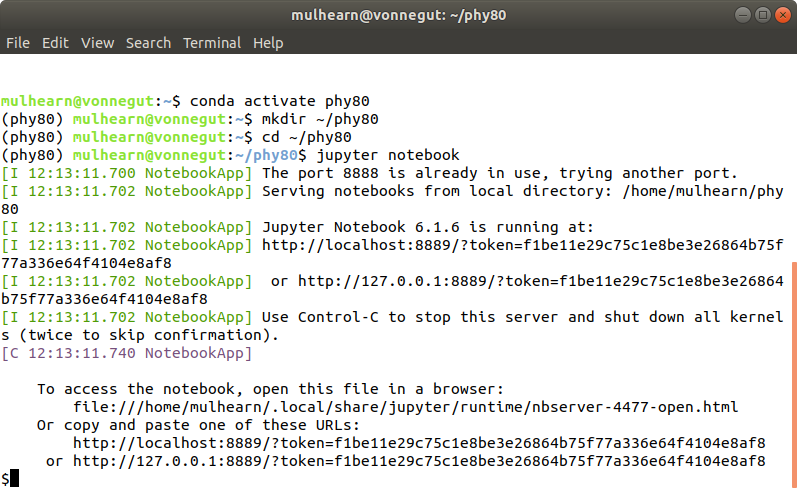
\includegraphics[width=0.65\textwidth]{figs/labs/python/jupyter_startup.png} 
\caption{Example starting Jupyter Notebook from the Linux command line.  In Windows, you will need to open the Anaconda Prompt instead of a terminal.}
\label{fig:jupyterstartup}
\end{center}
\end{figure}

\begin{figure}[htbp]
\begin{center}
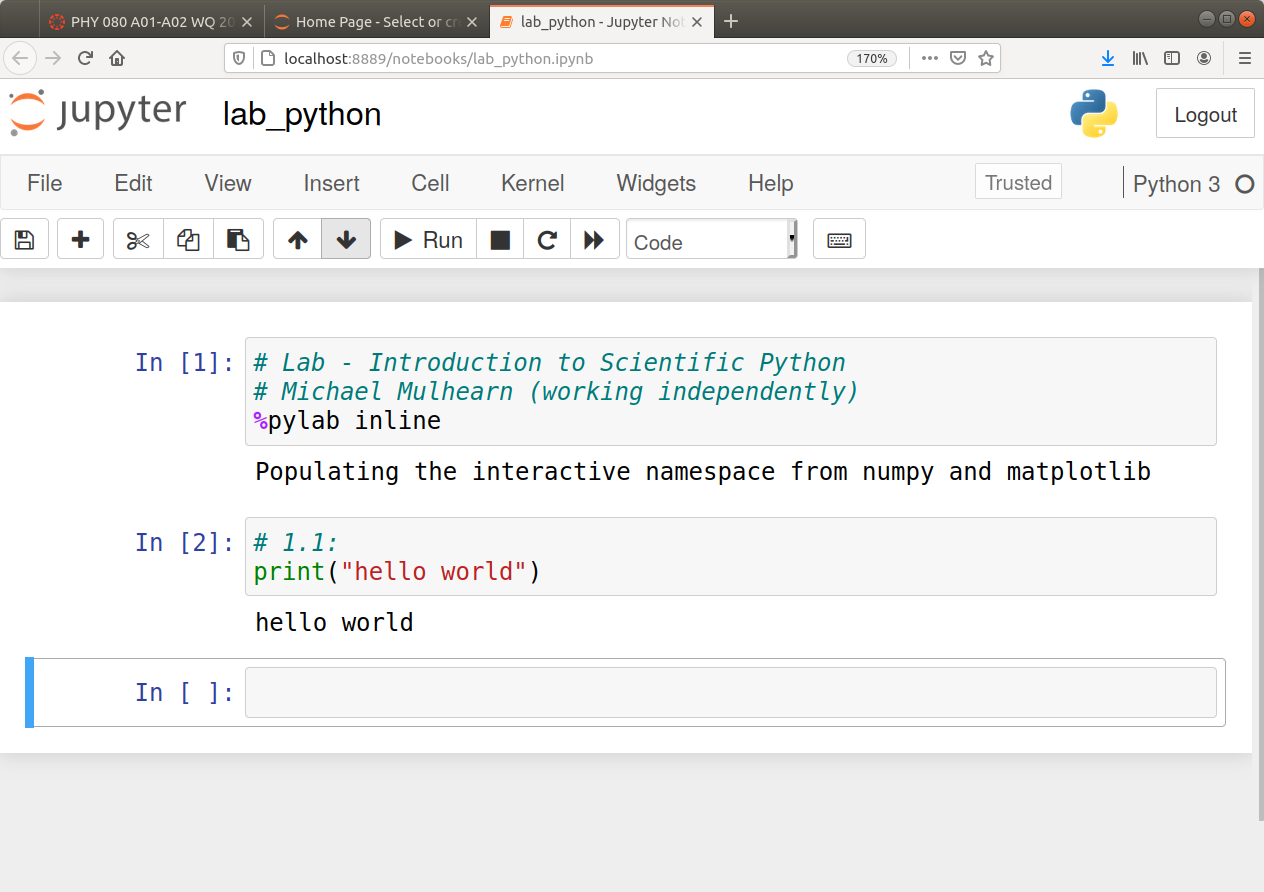
\includegraphics[width=0.65\textwidth]{figs/labs/python/jupyter_window.png} 
\caption{The Hello World example Jupyter Notebook.}
\label{fig:jupyterwindow}
\end{center}
\end{figure}

\begin{figure}[htbp]
\begin{center}
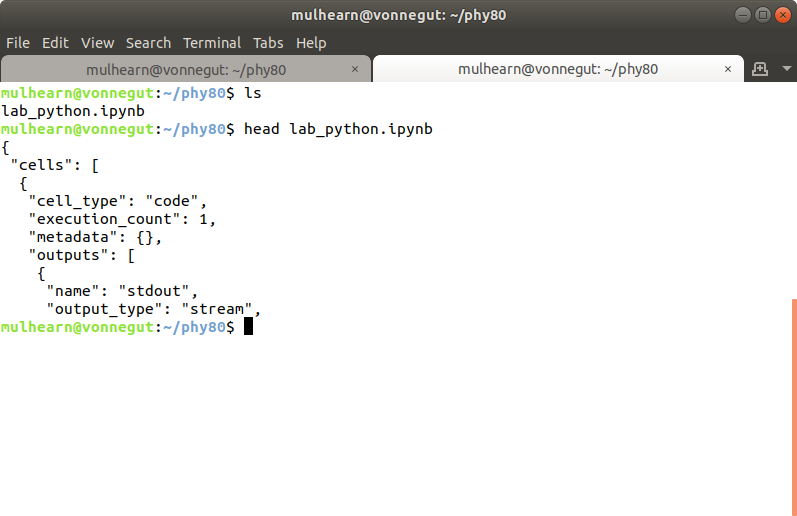
\includegraphics[width=0.65\textwidth]{figs/labs/python/jupyter_saved.png} 
\caption{Example showing the saved Jupyter notebook.  Notice that notebook file (ipynb) is not human readable on its own: it requires the Jupyter software to render it in a human readable form.}
\label{fig:jupytersaved}
\end{center}
\end{figure}

After following the software installation instructions on the course
website, activate the Physics 80 environment with:
\begin{verbatim}
$ conda activate phy80
\end{verbatim}
Then, navigate to a working directory for this session, and start the notebook with:
\begin{verbatim}
$ jupyter notebook
\end{verbatim}
This should start the Jupyter Notebook server and open a client in your web browser.
An example starting a Jupyter Notebook from Linux is shown in Fig.~\ref{fig:jupyterstartup}.

You should create one Jupyter Notebook per lab assignment, by choosing
the New (Python 3) option in your client.  Change the name of your
notebook to something that clearly identifies the lab.  Start each lab
with comments (starting with ``\#'' symbol) indicating the title of
the lab, then your name followed by your lab partners.  See the first
cell of Fig.~\ref{fig:jupyterwindow} for an example.  This first cell
is also a good place to issue the ipython ``magic function'':
\begin{verbatim}
%pylab inline
\end{verbatim}
which will setup the notebook for inline plots and load the numpy and matplotlib libraries for you.

Each assignment will consist of a number of steps, clearly numbered like this one, you first step:

\begin{plot}
Print ``hello world'' using the python print command.
\end{plot}
\noindent
To keep your notebook clear, label cells (such as this one) with a
comment for the assignment step number, as in the second cell of
Fig.~\ref{fig:jupyterwindow}.  You only need to label one cell if
the assignment is fullfilled across several cells.

Jupyter Notebook checkpoints your work automatically.  You should be
able to see your notebook saved in the working directory where you
started, as in Fig.~\ref{fig:jupytersaved}.  Notice that while the
notebook file is ASCII text, it is not a human readable format.  The
Jupyter software is needed to render the notebook in a human readable
way.  To make your grader's life easier, you will be submitting PDF
versions of your notebook, once all of the tasks are completed and the
output is visible.  There are several ways to make a PDF file from
your notebook, but the most reliable is to use the ``Print Preview''
option to view the notebook as a PDF file within your browser, then
use the print feature of your browser to print the page as a PDF file.
Try this now, and make sure you can create a legible PDF file, but do
not submit it to the course site, as you still have more to do.
Always keep your python notebook file (ipynb) even after you submit
the assignment.  If you have problems, you can reproduce a PDF file
from the notebook file, but it is tedious to reproduce your notebook
from PDF.  If you have problems producing the PDF file, you can submit
the ``ipynb'' file as a temporary work-around, but work with your TA
to sort out the problem as quickly as possible.

\section{Scientific Python lecture notes}

A link to the Scientific Python lecture notes is available on the
course website.  These lecture notes are a community-based effort
which is well-maintained and constantly improving.  This section
contains example problems designed to reinforce the key concepts from
the first chapter of the Scientific Python Lecture Notes (SPLN).
Nearly all of Chapter 1 is useful, but these examples single out the
most essential sections for getting started with compuation in this
course.

Read through SPLN 1.2.2 and complete the following exercises in your notebook:

\begin{plot}
  Make some of your own simple calculations demonstrating the use of
  integers, floats, and Boolean variables.  Make your own list of
  strings, and demonstrate a few list operations.
\end{plot}

\begin{plot}
\begin{samepage}  
Try to predict the output of this code snippet:
\begin{verbatim}
a=3
b=a
a=2 #update
print(b)
\end{verbatim}
\end{samepage}
Run the code and check the output.  Are integers mutable or immutable?
At the line marked \#update, is a being changed by assignment or modification in place?
\end{plot}

\begin{plot}
Try to predict the output of this code snippet:
\begin{verbatim}
a=[3]
b=a
a[0]=2 #update
print(b[0])
\end{verbatim}
Run the code and check the output.  What type of data format is $a$?
Is that a mutable data type?  At the line marked \#update, is $a$
being changed by assignment or by modification in place?  Change that
line so as to do the opposite.  Does the program output change?
\end{plot}

Read through SPLN 1.2.3 and complete the following exercises in your notebook:

\begin{plot}
Use a for loop to print the first 10 powers of 3:  1,3,9,27,...
\end{plot}

\begin{plot}
Use a while loop to find the first number n for which the sum $1^2+2^2+3^2+...+n^2$ exceeds 1000.
\end{plot}

\begin{plot}
Use a for loop to calculate $n!$ by simply multiplying every value from $n$ to 1.
\end{plot}

\begin{plot}
Write a program to calculate and list the first 10 prime numbers after
100.  Use only basic python features such as while loops, for loops,
conditionals, assignment(=), equality (==), multiplication (*), and
the integer divide operation (//).  Do not use the mod operation (\%).
\end{plot}

Read through SPLN 1.4.1.1-3, 1.4.1.5 and complete the following problems:

\begin{plot}
Use the np.arange to define a 1-D numpy array of integers from 10 to
30 (inclusive).  Uses slices to print (a) every third element
(10,13,..), (b) the last five elements (26,27,...,30), and (c) every
other element in reverse order (30, 28, 26, ..., 10).
\end{plot}

\begin{plot}
Define variables $a$ and $b$ as numpy arrays of floats each of length
three.  Write a code snippet to calculate and print the vector dot
product of $a \cdot b$ using an explicit for loop, i.e. loop over
indexes 0,1,2 and increment a sum by the product.  This is how you
write this program in a language such a C.  Now use the python * and
np.sum operation to compute the dot product in a single line, with no
explicit for loop.  The elimination of tedious explicit for loops is
why programming in Scientific Python is much more fun than any other
common language, once you get used to the idea.
\end{plot}

The Scientific Python Lecture Notes are an excellent resource.  These
examples and sections are a good starting point for the work we will
be doing in this course, but remember that there is much more
available for you to refer to in the future!

\section{Submitting your assignment}

Before submitting, take some time to clean up your assignments to
remove anything superfluous and place the exercises in the correct
order.  You can also add comments as needed to make your work clear.
You can use the Cell $\to$ All Output $\to$ Clear and Cell $\to$ Run
All commands to make sure that all your output is up to date with the
cell source.

When you are satisfied with your work, print the PDF file as described
earlier and submit it to the course website.

